\scanpage{62}
\figure{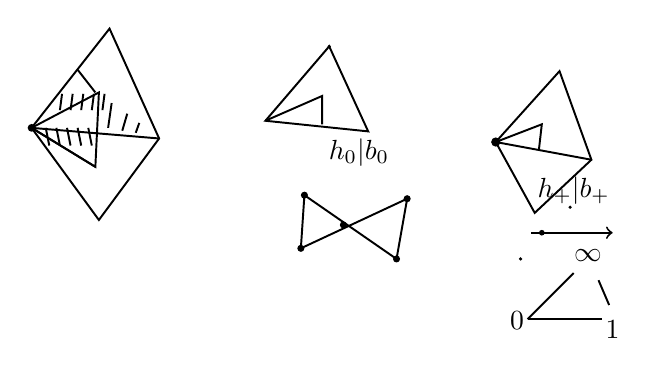
\begin{tikzpicture}[x=.9cm,y=.9cm,line width=.7pt]
\draw(0,1.6)--(1.1,3)--(1.8,1.45)--(.95,.3)--cycle;\draw(0,1.6)--(1.8,1.45);\draw(0,1.6)--(.95,2.1)--(.9,1.05)--cycle;\draw(.65,2.42)--(.9,2.1);\draw(0,1.6)--(.9,1.05);\foreach \x in {.2,.35,.5,.65,.8}{\draw(\x,1.6)--(\x+.05,1.35);\draw(\x+.2,1.85)--(\x+.23,2.08);} \draw(1.08,1.6)--(1.13,1.95);\draw(1.28,1.56)--(1.35,1.8);\draw(1.47,1.53)--(1.52,1.67);\fill(0,1.6)circle(.055);
\draw(3.3,1.7)--(4.2,2.75)--(4.75,1.55)--cycle;\draw(3.3,1.7)--(4.1,2.05)--(4.1,1.65);\fill(4.2,2.75)circle(.025);\node at(4.62,1.25){$\unsure{h_0|b_0}$};
\draw(3.85,.65)--(3.8,-.1)--(5.3,.6)--(5.15,-.25)--cycle;\foreach\x/\y in{3.85/.65,3.8/-.1,4.4/.23,5.3/.6,5.15/-.25}{\fill(\x,\y)circle(.05);}
\draw(6.55,1.4)--(7.45,2.4)--(7.9,1.15)--(7.1,.4)--cycle;\draw(6.55,1.4)--(7.9,1.15);\draw(6.55,1.4)--(7.2,1.65)--(7.16,1.3);\fill(6.55,1.4)circle(.065);\node at(7.65,.72){$\unsure{h_+|b_+}$};\draw[->](7.05,.12)--(8.2,.12);\fill(7.2,.12)circle(.04);\fill(6.9,-.25)circle(.025);\fill(7.6,.48)circle(.025);
\draw(7,-1.1)--(8.05,-1.1);\draw(7,-1.1)--(7.65,-.45);\draw(8,-.55)--(8.15,-.9);\node at(6.85,-1.12){$0$};\node at(7.85,-.2){$\infty$};\node at(8.2,-1.25){$1$};
\end{tikzpicture}}

\diagram{\begin{tikzcd}[ampersand replacement=\&]\mathbb Z/5\mathbb Z\arrow[d]\\D_5\end{tikzcd}}
($D_5\times\mathbb Z/2\mathbb Z$ dans \unsure{théo. non orientée}
\figure{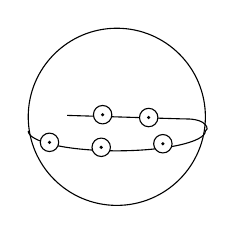
\begin{tikzpicture}[scale=.9]
\draw(0,0)circle(1.25);\draw(-1.25,-.2)arc(180:360:1.25 and .28);\draw(-.7,.02)--(.95,-.03)..controls(1.3,-.02)and(1.3,-.2)..(1.25,-.2);
\foreach\x/\y in{-.95/-.36,-.22/-.43,.65/-.38,-.2/.03,.45/-.01}{\draw[fill=white](\x,\y)circle(.13);\fill(\x,\y)circle(.025);}
\end{tikzpicture}}
12 possibilités \deleted{\unsure{K}} (struct. pentag. sur $K$)

(\uline{NB} \deleted{\unsure{les}} 12 sommets de l'icos. le stabilisateur d'un sommet est $\mathbb Z/5\mathbb Z$, \deleted{\unsure{d'ordre $\mathbb Z/5\mathbb Z$}} \inserted{et dans le cas non orienté} $D_5$)
\margin{\uline{Implique \unsure{orientation} de $K$}}

$\mathbb Z/4\mathbb Z$

($D_4$ dans théorie non orientée)
\figure{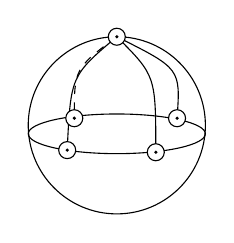
\begin{tikzpicture}[scale=.9]
\draw(0,0)circle(1.25);\draw(0,-.12)ellipse(1.25 and .28);\draw(0,1.25)..controls(-.65,.7)..(-.7,-.35);\draw(0,1.25)..controls(.9,.8)..(.85,.1);\draw(0,1.25)..controls(.55,.7)..(.55,-.38);\draw[dashed](0,1.25)..controls(-.6,.8)..(-.6,.1);
\foreach\x/\y in{0/1.25,-.6/.1,.85/.1,-.7/-.35,.55/-.38}{\draw[fill=white](\x,\y)circle(.12);\fill(\x,\y)circle(.025);}
\end{tikzpicture}}
$30=15\times2$ possibilités (\inserted{\uline{structure en}} carrés orientés dans $K$)

(\uline{NB} 30 arêtes de l'icosaèdre, le stabilisateur d'un sommet est $\mathbb Z/2\mathbb Z$ (et $D_2=\mathbb Z/2\times\mathbb Z/2$ au cas non orienté)

\uline{n'implique pas d'orientation de $K$}

\diagram{\begin{tikzcd}[ampersand replacement=\&]\mathbb Z/3\mathbb Z\arrow[d]\\\unsure{\mathfrak S_3|G_3}\end{tikzcd}}
($D_3\times\mathbb Z/2\mathbb Z$ en théorie non orientée
\figure{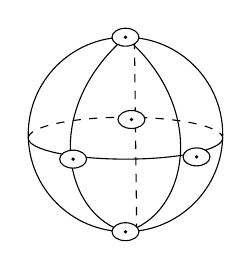
\begin{tikzpicture}[scale=.95]
\draw(0,0)circle(1.3);\draw(-1.3,-.05)arc(180:360:1.3 and .28);\draw[dashed](-1.3,-.05)arc(180:0:1.3 and .28);\draw(0,1.3)..controls(-1.15,.3)and(-.8,-1.1)..(0,-1.3);\draw(0,1.3)..controls(1.15,.3)and(.8,-1.1)..(0,-1.3);\draw[dashed](.12,1.25)--(.15,-1.25);
\foreach\x/\y in{0/1.3,.08/.2,-.7/-.33,.95/-.3,0/-1.3}{\draw[fill=white](\x,\y)ellipse(.18 and .12);\fill(\x,\y)circle(.025);}
\end{tikzpicture}}
$20=10\times$ possibilités (triangles de $K$ \deleted{\unsure{pas de nature}} \inserted{orientés} de $K$) (NB 20 faces de l'icosaèdre, stabilisateur de chacune est $\mathbb Z/3\mathbb Z$ ; groupe $\unsure{\mathfrak S_3|G_3}$ cas non orienté)
\mspage{61}
